
\section{\trGradient，\trFloerEquation}
\label{sec:gradient-floer-equation}

正如在\trMorse{}情形中那样，我们需要一个\trVectorField（其诸\trTrajectory{}将定义这个\trComplex{}的\trDifferential）。我们将对\trContractible\trLoop{}所成空间 $\scr{L}W$ 上的一个特定\trMetric{}使用\trGradient。当心，\trGradient{}是依赖于\trMetric{}的；倘若需要改动\trVectorField（想想第 2 章中的\trSmale{}性质），我们所拥有的那份灵活性，就将通过诸\trMetric（从而通过诸\trAlmostComplex{}结构）来获得。

让我们先取定 $W$ 上一个被 $\omega$ \trCalibrated{}的\trAlmostComplex{}结构 $J$（见\cref{sec:complex-structures}）。它在 $W$ 上定义了一个\trRiemann\trMetric{} $g$，即
\[
g(X,Y)=\omega\bigl(X,J(Y)\bigr)\text{。}
\]
这在 $\scr{L}W$ 上诱导了一个\trMetric，定义为
\[
\langle Y,Z\rangle=\int_0^1g\bigl(Y(t),Z(t)\bigr)\,dt
\]
（此处 $Y$ 与 $Z$ 表示沿一条\trLoop{} $x$ 定义的\trVectorField）。显然，这个公式定义了一个\trSymmetricBilinearForm；由于 $g_t$ 是\trPositiveDefinite{}的，这个形式也等于
\[
\langle Y,Y\rangle=\int_0^1g\bigl(Y(t),Y(t)\bigr)\,dt\ \ge\ 0\text{，}
\]
而等号成立当且仅当 $Y=0$，从而 $\langle\cdot,\cdot\rangle$ 是\trPositiveDefinite{}的。它也可以写作
\[
\langle Y,Z\rangle=\int_0^1\omega_{x(t)}\bigl(Y(t),J(Z(t))\bigr)\,dt\text{。}
\]

若 $f\colon\scr{L}W\to\RR$ 是一个函数，那么它的\trGradient{}就是由
\[
\begin{aligned}
\langle\operatorname{grad}_x f,Y\rangle_x
&=\int_0^1g_t\bigl((\operatorname{grad}_x f)(t),Y(t)\bigr)\,dt\\
&=\int_0^1\omega_{x(t)}\bigl((\operatorname{grad}_x f)(t),JY(t)\bigr)\,dt=(df)_x(Y)
\end{aligned}
\]
所定义的\trVectorField{} $\operatorname{grad}f$。

由于我们还有
\[
(d\scr{A}_H)_x(Y)=\int_0^1\omega_{x(t)}\bigl(\dot{x}(t)-X_t(x),Y(t)\bigr)\,dt
\]
（参见\cref{subsec:action-functional-b}），故 $\scr{A}_H$ 的\trGradient{}便是
\[
-\scr{X}_H(t)=(\operatorname{grad}_x\scr{A}_H)(t)=J_{x(t)}\bigl(\dot{x}(t)\bigr)+\operatorname{grad}_{x(t)}H_t
\]
（$H_t$ 的\trGradient{}是就\trMetric{} $g$ 计算的）。

\setcounter{figure}{3}%
\begin{figure}[htbp]
\centering
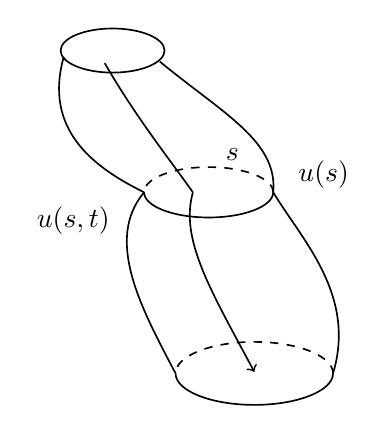
\begin{tikzpicture}[line width=0.6pt,scale=1.0]
  \draw (-0.9,3.3) ellipse (0.66 and 0.28);
  \draw[dashed] (1.14,1.5) arc (0:180:0.82 and 0.32);
  \draw (-0.5,1.5) arc (180:360:0.82 and 0.32);
  \draw[dashed] (1.9,-0.8) arc (0:180:1.0 and 0.4);
  \draw (-0.1,-0.8) arc (180:360:1.0 and 0.4);
  \draw (-1.52,3.22) .. controls (-1.78,2.3) and (-1.15,1.82) .. (-0.5,1.5);
  \draw (-0.5,1.5) .. controls (-1.0,0.9) and (-0.55,0.05) .. (-0.1,-0.8);
  \draw (-0.3,3.16) .. controls (0.5,2.5) and (1.2,2.15) .. (1.14,1.5);
  \draw (1.14,1.5) .. controls (1.5,0.9) and (2.2,0.2) .. (1.9,-0.8);
  \draw (-1.0,3.14) .. controls (-0.6,2.45) and (-0.2,1.95) .. (0.12,1.5);
  \draw[->] (0.12,1.5) .. controls (-0.05,0.9) and (0.35,0.25) .. (0.9,-0.78);
  \node at (1.78,1.72) {$u(s)$};
  \node at (-1.4,1.14) {$u(s,t)$};
  \node at (0.62,1.98) {$s$};
\end{tikzpicture}
\caption{}
\label{fig:solution-cylinder-sections}
\end{figure}

而\trVectorField{} $\scr{X}=\scr{X}_H$（即负\trGradient，为与前几章保持一致）的诸\trTrajectory{}因而是形如
\[
\begin{aligned}
\RR&\longrightarrow\scr{L}W\\
s&\longmapsto u(s)
\end{aligned}
\]
（其中理解为：对每个 $s$，$u(s)$ 是一条\trLoop，其在时刻 $t$ 的值将记作 $u(s,t)$）的下述\trDifferential{}方程的解：
\[
\frac{\partial u}{\partial s}=-J_{u(s,t)}\Bigl(\frac{\partial u}{\partial t}\Bigr)-\operatorname{grad}_{u(s,t)}H_t\bigl(u(s,t)\bigr)
\]
……或者，更简洁地，是下述（偏）\trDifferential{}方程的解：
\[
\frac{\partial u}{\partial s}+J(u)\frac{\partial u}{\partial t}+\operatorname{grad}H_t(u)=0\text{。}
\]
这条方程就是\emph{\trFloerEquation}。回想一下，使我们感兴趣的，乃是它在 $t$ 上\trPeriodic{}为 $1$ 的那些 $\cC^\infty$ \trContractible{}解。

\begin{remark}\label{thm:floer-equation-remarks}
\begin{enumerate}[label=(\arabic*)]
\item 若 $H$ 不依赖于 $t$，那么同样不依赖于 $t$ 的那些解 $u$ 满足
\[
\frac{du}{ds}+\operatorname{grad}H(u)=0\text{。}
\]
这些就是 $H$ 的（负）\trGradient{}的诸\trTrajectory。
\item 一般地，不依赖于 $s$ 的那些解 $u$ 满足
\[
\frac{\partial u}{\partial t}=J(u)\operatorname{grad}H_t(u)=X_t(u)\text{。}
\]
这就是那个（意料之中的）事实：\trGradient{}之流的诸\trStationary{}\trTrajectory，正是\trHamiltonian{}系统的诸\trPeriodic{}解。
\item 若 $H_t\equiv 0$，那么这条方程就简单地是
\[
\frac{\partial u}{\partial s}+J(u)\frac{\partial u}{\partial t}=0\text{；}
\]
这就是\trCauchyRiemann{}方程。这时我们便把 $(s+it)\mapsto u(s,t)$ 称为一条\emph{$J$-\trHolomorphic{}曲线}。
\end{enumerate}
\end{remark}
